\section{Реализация}

\subsection{Объектно-ориентированное проектирование}

Перед началом реализации необходимо провести объектно-ориентированное проектирование системы. Данный этап подразумевает представление бизнес
логики в виде программных функций и разнесение этих функций по классам. Таким образом в программе формируется слой бизнес-логики. В данной 
случае этот слой было решено реализовать в виде набора сервисов. Наполнение классов осуществлялось так, чтобы соблюдались основные
принципы проектирования, такие, например, как принцип единственной ответственности (single responsibility principle). Результаты 
проектирования представлены ниже, на рисунке \ref{fig:02-bl} в виде UML диаграмы. 

\begin{figure}[H]
    \centering
    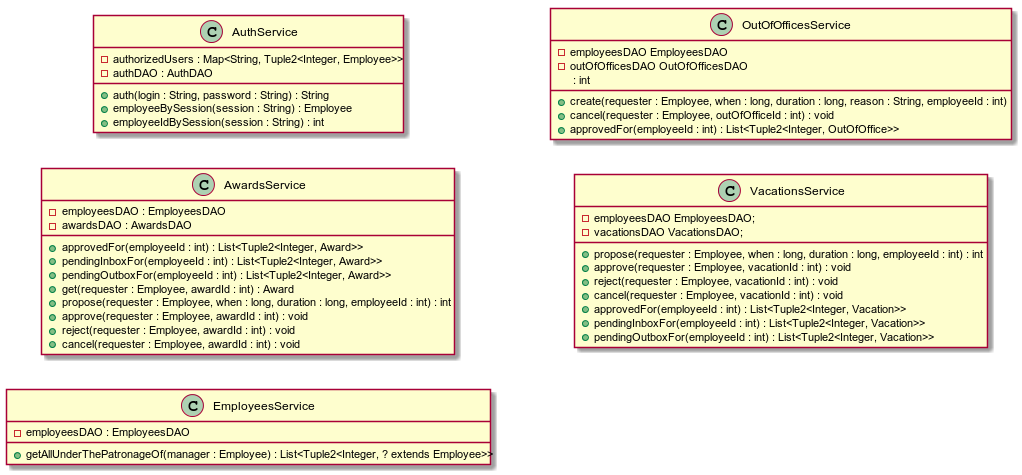
\includegraphics[width=\textwidth]{resources/02_implementation/01_bl.png}
    \caption{Модель предметной области системы}
    \label{fig:02-bl}
\end{figure}

Как видно, в результате проектирования было выделено $5$ сервисов. Каждый из классов параметризуется только лишь объектами доступа к данным
(DAO --- data access object) соответствующего типа. Приведем краткий разбор данных классов:

\begin{itemize}
    \item \code{AuthService} отвечает за авторизацию и аутентификацию пользователей, а также за выделение им специальных сессионных ключей.
    \begin{itemize}
        \item Процедура \code{auth} отвечает за выделение и сохранение сессионного ключа пользователю с заданными логином и паролем.
        \item Процедура \code{employeeBySession} отвечает за выдачу сущности пользователя по сессионному ключу.
        \item Процедура \code{employeeIdBySession} отвечает за выдачу идентификационного номера сущности пользователя по сессионному ключу.
    \end{itemize}
    \item \code{AwardsService} предназначен для работы с премиями.
    \begin{itemize}
        \item Процедура \code{approvedFor} предназначена для выдачи премий заданного пользователя, которые уже были подтверждены 
            бухгалтером. 
        \item Процедура \code{pendingInboxFor} предназначена для выдачи запросов на выплату премий, направленных заданному пользователю с
            ролью <<бухгалтер>>.
        \item Процедура \code{pendingOutboxFor} предназначена для для выдачи запросов на выплату премий, отправленных заданным 
            пользователем с ролью <<менеджер>>. 
        \item Процедура \code{get} выдает сущность-премию по ее идентификационному номеру. При этом осуществляется проверка прав доступа
            пользователя \code{requester} на доступ к заданной сущности.
        \item Процедура \code{propose} предназначена для создания запроса на выдачу премии заданному пользователю в заданный срок и с 
            заданным размером. При этом осуществляется проверка прав доступа пользователя \code{requester} на создание такого запроса с 
            указанным получателем.
        \item Процедура \code{approve} предназначена для подтверждения заданного запроса на выдачу премии. При этом осуществляется проверка 
            прав доступа пользователя \code{requester} на выполнение данного действия.
        \item Процедура \code{reject} предназначена для отклонения заданного запроса на выдачу премии. При этом осуществляется проверка 
            прав доступа пользователя \code{requester} на выполнение данного действия.
        \item Процедура \code{cancel} отменяет запрос на выдачу премий, который еще не был ни подтвержден, ни отклонен. При этом     
            осуществляется проверка прав доступа пользователя \code{requester} на выполнение данного действия.
    \end{itemize}
    \item \code{OutOfOfficeService} предназначен для работы с отсутствиями на рабочем месте.
    \begin{itemize}
        \item Процедура \code{create} предназначена для резервирования времени отсутствия в офисе в заданный период и с указанной причиной.
            При этом осуществляется проверка прав доступа пользователя \code{requester} на создание такого запроса с указанным получателем.
        \item Процедура \code{cancel} предназначена для отмены резервации времени нахождения вне офиса. При этом осуществляется проверка 
            прав доступа пользователя \code{requester} на выполнение данного действия.
        \item Процедура \code{approvedFor} предназначена для извлечения всех резерваций времени на отсутствие в офисе для указанного 
            пользователя.
    \end{itemize}
    \item \code{VocationService} предназначен для работы с отпусками. Здесь мы не будем приводить более подробный разбор методов данного 
        класса, поскольку все они аналогичны уже рассмотренным методам из класса \code{AwardsService}.
    \item EmployeeService отвечает за работу с пользователями.
    \begin{itemize}
        \item Процедура \code{getAllUnderThePatronageOf} отвечает за выдачу пользователей, которые подотчетны указанному пользователю.
    \end{itemize}
\end{itemize}

Также в рамках этапе объектно-ориентированного проектирования был создан набор диаграмм последовательностей в нотации UML (sequence duagram).
Ниже, на рисунках \ref{fig:02-propose-award} -- \ref{fig:02-decline-award} представлено несколько таких диаграмм для операций создания,
подтверждения и отклонения заявки на выдачу премии соответственно.

\begin{figure}[H]
    \centering
    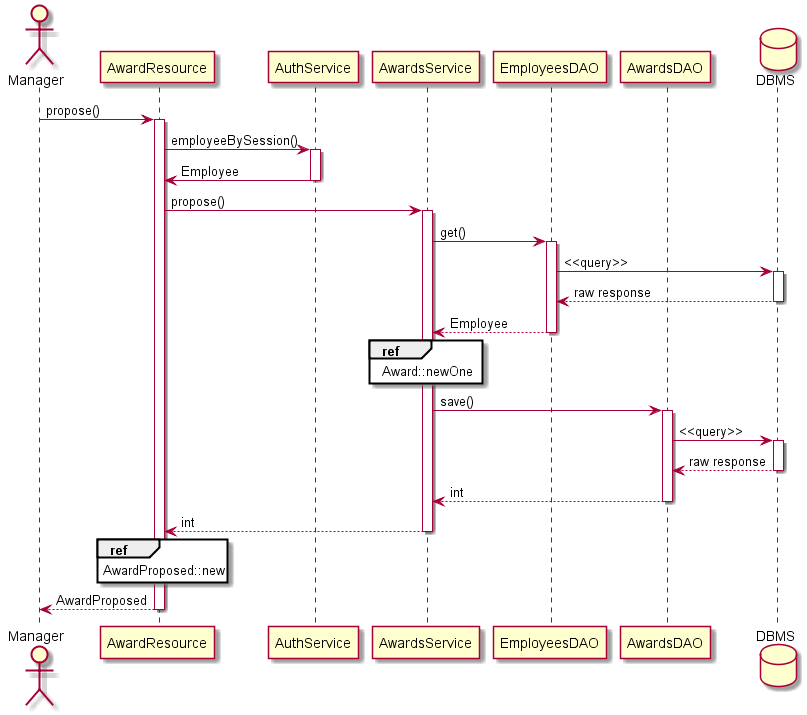
\includegraphics[width=\textwidth]{resources/02_implementation/02_award_employee.png}
    \caption{Процесс создания заявки на премирование}
    \label{fig:02-propose-award}
\end{figure}

\begin{figure}[H]
    \centering
    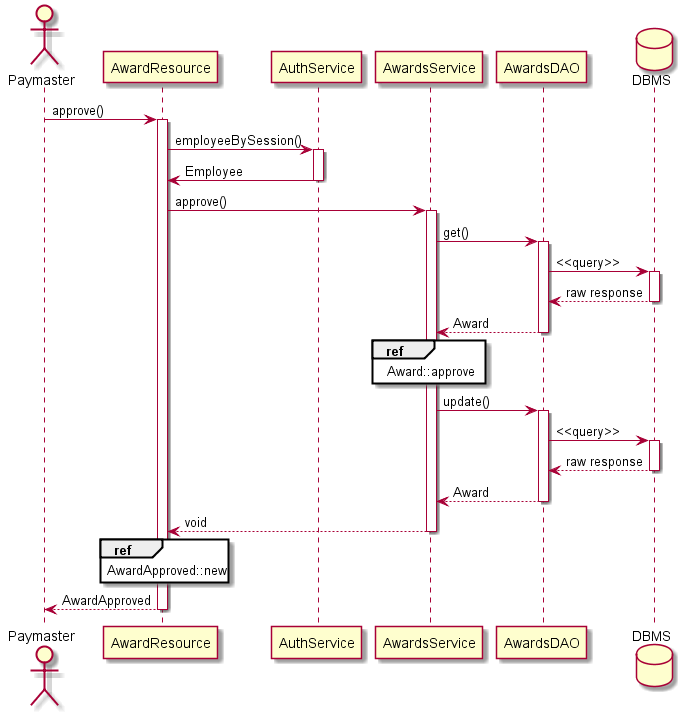
\includegraphics[width=0.55\textwidth]{resources/02_implementation/03_accept_award.png}
    \caption{Процесс подтверждения заявки на премирование}
    \label{fig:02-accept-award}
\end{figure}

\begin{figure}[H]
    \centering
    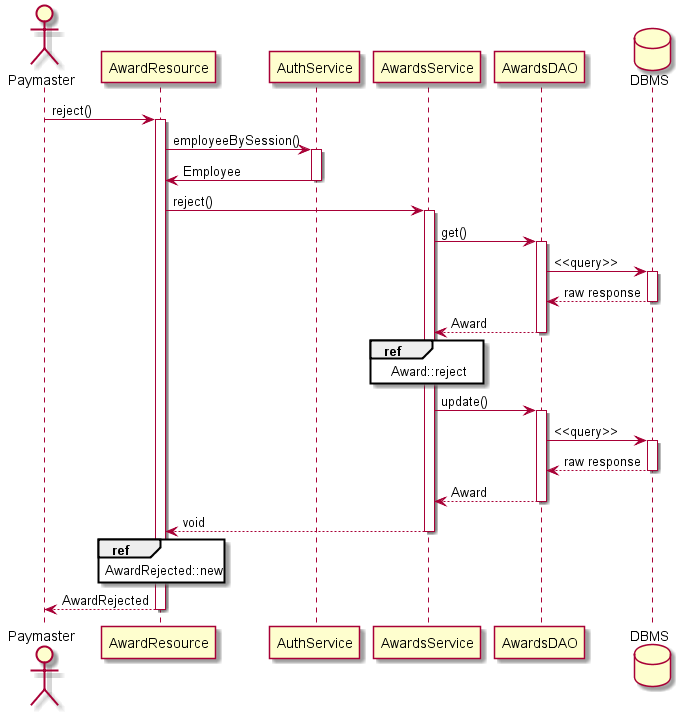
\includegraphics[width=0.55\textwidth]{resources/02_implementation/04_decline_award.png}
    \caption{Процесс отклонения заявки на премирование}
    \label{fig:02-decline-award}
\end{figure}

\subsection{Детали реализации}

Разработанное приложение необходимо реализовать в виде сетевого (web based) приложения. По этой причине, помимо уровня бизнес логики был 
также выделен уровень представления приложения, отвечающий за принятие запросов от клиента и отправку ему ответов. Методы, реализуемые на 
данном уровне, работают почти одинаково по следующей схеме:
\begin{itemize}
    \item Аутентификация пользователя путем обращения к экземпляру класса \code{AuthService}.
    \item Преобразование аргументов сетевого запроса к виду, удобному для уровня бизнес логики.
    \item Преобразованный запрос направляется на уровень бизнес логики, в соответствующий сервис.
    \item Результат, полученный от сервиса преобразуется к виду, удобному для ответа клиенту. 
\end{itemize}
Такая логика работы позволяет обеспечить независимость уровня бизнес логики от уровня представлений и, как следствие, большую гибкость. 
Другими словами, сервисные классы не имеют понятия о том, что приложение является сетевым, что позволяет переиспользовать данный код
при разработке, например, обычного (desktop) приложения. В то же время, любые изменения на уровне представления не затрагивают сервисный
уровень и, следовательно, не могут его <<сломать>>. Классы на уровне представления реализованы с учетом методики REST. Данный 
предоставляются в формате json. Преобразование объектов в формат json осуществляется при помощи библиотеки \code{jackson}. 

Из рисунка \ref{fig:02-bl} видно, что на уровне бизнес логики используются специальный объекты доступа к данным. Данные объекты также 
располагаются на отдельном уровне приложения --- уровне доступа к данным. Принцип работы методов, расположенных на данном уровне, совпадает
с логикой работы методов на уровне представления с той лишь только разницей, что здесь опускается этап аутентификации пользователей. 
Таким образом, обеспечивается такая же гибкость взаимоотношения между уровнями бизнес логики и доступа к данным, как и в случае уровней
представления данных и бизнес логики. Для реализации данного уровня использовалась библиотека \code{ebean-orm}, осуществляющая 
преобразование сущностей базы данных в программные сущности (object relational mapping). 

Также стоит отметить, что для избежания различных проблем, связанных с проектирование программного обеспечения, и для обеспечения 
гибкости в ходе реализации приложения была использована библиотека, осуществляющая внедрение зависимостей (dependency injection), --- 
\code{Guice}. Также для борьбы с кончервативным кодом (boilerplate code) была использована библиотека \code{lombok}.

\subsection{Методика и результаты тестирования}

На этапе тестирования использовались библиотеки \code{junit} и \code{mockito}. Использование данных библиотек позволило реализовать тесты
в соответствии с лучшими практиками. Отметим, что тестирование проводилось только для уровня бизнес логики. В силу большого количества
тестов и проверяемых в них условиях в рамках данной работы не будет приводиться сколь-нибудь подробное описание тестовых методов. Вместо
этого представим отчет по тестированию, сгенерированные при помощи утилиты \code{maven} и интегрированной среды разработки 
\code{IntelliJ IDEA}.

\begin{center}
    \inputminted{console}{resources/02_implementation/05_tests}
    \captionof{listing}{Отчет по тестированию, сгенерированный в \code{maven}}
\end{center}

\begin{figure}[H]
    \centering
    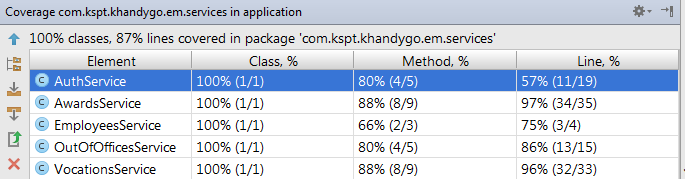
\includegraphics[width=\textwidth]{resources/02_implementation/06_tests.png}
    \caption{Отчет по тестированию, сгенерированный в \code{IntelliJ IDEA}}
    \label{fig:02-test}
\end{figure}

\subsection{Инструкция системного администратора}

Для развертывания приложения необходимы следующие системные компоненты:
\begin{itemize}
    \item Сервер \code{MySQL} версии $5.5$ или выше.
    \item Утилита \code{maven} версии $3.1.0$ или выше.
    \item Сервер приложений \code{wildfly} версии $10.1.0$ или выше.
\end{itemize}
Теперь необходимо настроить \code{MySQL} сервер следующим образом:
\begin{itemize}
    \item Порт $3307$.
    \item Создать схему с именем \code{test}.
    \item Наполнить базу данных так, как показано в листинге \ref{lst:02-mysql-create}. 
    \item Создать пользователя с логином \code{em\_admin} и паролем \code{1234}.
    \item Выделить пользователю \code{em\_admin} права на чтение и запись в схеме \code{test}.
\end{itemize}
Никакой дополнительной настройки \code{maven} и \code{wildfly} не требуется. Для запуска сервера приложений в простейшем случае можно
воспользоваться скриптом \code{standalone} (расширение \code{.bat} или \code{.sh} зависит от используемой операционной системы и средств),
расположенным в директории \code{bin}. Теперь для размещения проекта на сервере необходимо выполнить команду \code{mvn clean install 
wildfly:deploy} из директории проекта. Здесь, конечно, предполагается, что на рабочей машине есть доступ к сети Интернет.

\begin{center}
    \inputminted[lastline=34]{sql}{resources/02_implementation/07_mysql_create}
    \inputminted[firstline=35]{sql}{resources/02_implementation/07_mysql_create}
    \captionof{listing}{Скрипт создания базы данных приложения \label{lst:02-mysql-create}}
\end{center}

Для создания пользователя системы необходимо выполнить в \code{MySQL} команду вида
\begin{center}
    \sql{INSERT INTO users VALUES(null, login, MD5(pswd), name, m_id, p_id);},
\end{center}
где: \code{login} --- логин пользователя, \code{pswd} --- пароль пользователя, \code{name} --- имя пользователя, \code{m\_id} и 
\code{p\_id} --- идентификационные номера менеджера и бухгалтера данного пользователя соответственно. 

В случае правильной настройки всех компонент приложение должно быть доступно по адресу сервера приложений на порте с номером $8080$
с добавлением \code{/application}.

\subsection{Инструкция пользователя}

Для того, чтобы начать пользоваться системой необходимо сначала пройти аутентификацию на заглавной странице. Для этого в соответствующие 
поля вводятся логин и пароль пользователя. Далее, в левой части экрана будет доступно меню. 
\begin{itemize}
    \item Для того, чтобы просмотреть подтвержденные заявки на отпуск и выплату премии необходимо перейти по пункту \code{Home}.
    \item Для того, чтобы просмотреть информацию о своем менеджере и бухгалтере, необходимо перейти по пункту \code{Stuff}.
    \item Для того, чтобы просмотреть информацию об отправленных, но еще не подтвержденных и не отклоненных заявках, а также заявках,
        направленных данному пользователю, необходимо перейти по вкладке \code{Proposals}.
    \item Для того, чтобы отправить заявку на предоставление отпуска необходимо нажать кнопку \code{Propose Vacation}.
    \item Для того, чтобы зарезервировать время отсутствия в офисе необходимо нажать кнопку \code{Reserve Out Of Office}.
\end{itemize}
